\section[Statistical Entropy]{Statistical Entropy}

\begin{frame}{Statistical Entropy}
	Before discussing decision trees, we will take a detour into the key concept of \textbf{statistical entropy}:
	
	\begin{itemize}
		\item It is crucial for decision trees.
		\pause
		\item It is essential for logistic regression, as we have already seen.
		\pause
		\item But it is also vital for neural networks, which we have yet to cover!
	\end{itemize}
\end{frame}

\subsection[Surprise]{Surprise}

\begin{frame}{A Coin-Flipping Example}
	Let us consider a simple example. We have an unfair coin. The probabilities of getting "Heads" or "Tails" on a flip $X$ are as follows:
	\begin{equation*}
		\begin{cases}
			P(X = \text{"Heads"}) = 0 \\
			P(X = \text{"Tails"}) = 1
		\end{cases}
	\end{equation*}
	\pause
	\begin{itemize}
		\item I flip this coin once, and the result is "Tails".
		\item Nothing \textbf{surprising} here.
	\end{itemize}
\end{frame}

\begin{frame}{A Coin-Flipping Example}
	The probabilities of the coin are now changed, and we have the following instead:
	\begin{equation*}
		\begin{cases}
			P(X = \text{"Heads"}) = 0.1 \\
			P(X = \text{"Tails"}) = 0.9
		\end{cases}
	\end{equation*}
	\pause
	\begin{itemize}
		\item I flip this coin once, and the result is "Tails".
		\item This result is not very surprising, but still slightly more so than in the previous example.
	\end{itemize}
\end{frame}

\begin{frame}{A Coin-Flipping Example}
	\begin{itemize}
		\item The lower the probability $P(X = \text{"Tails"})$, the greater the \textbf{surprise} when the flip results in "Tails".
		\pause
		\item How can we express surprise based on probability?
	\end{itemize}
	\pause
	A first attempt, denoting surprise as $I$, could be:
	\begin{equation*}
		I(\text{"Tails"}) = \frac{1}{P(X = \text{"Tails"})}
	\end{equation*}
	\pause
	\begin{itemize}
		\item The lower the probability, the greater the surprise.
		\pause
		\item However, if the probability $P(X = \text{"Tails"}) = 1$, then the surprise is $I(\text{"Tails"}) = 1$.
		\pause
		\item It would seem more natural for the surprise to be zero if the event is certain.
	\end{itemize}
\end{frame}

\begin{frame}{Surprise or Information}
	\begin{block}{Definition: Surprise or Information}
		In his information theory, Claude Shannon defined the concept of \textbf{surprise}, also called \textbf{information} and denoted by $I$, as the logarithm of the inverse of the probability $P$ of an event $x$:
		\begin{equation*}
			I(x) = \log{\left(\frac{1}{P(X = x)}\right)} = - \log{P(X = x)}
		\end{equation*}
		In this equation, $x$ represents the realization of a random variable $X$.
		
		\vspace{0.3cm}
		\hfill
		\textit{--- Claude Shannon (1948)}
	\end{block}
	\pause
	Thanks to the use of the logarithm:
	\begin{itemize}
		\item The surprise is always very high when the probability becomes low.
		\item The surprise is now equal to 0 when the probability becomes equal to 1.
	\end{itemize}
\end{frame}

\begin{frame}{Surprise of Two Independent Events}
	Suppose the probabilities of our coin are now as follows:
	\begin{equation*}
		\begin{cases}
			P(X = \text{"Heads"}) = 0.2 \\
			P(X = \text{"Tails"}) = 0.8
		\end{cases}
	\end{equation*}
	\pause
	I perform 2 successive and \textbf{independent} flips and obtain the following result: $\{\text{"Tails"}, \text{"Heads"}\}$. What is the surprise associated with these flips?
	\begin{equation*}
		P(X_1 = \text{"Tails"}, X_2 = \text{"Heads"}) = P(X_1 = \text{"Tails"}) P(X_2 = \text{"Heads"})
	\end{equation*}
\end{frame}

\begin{frame}{Surprise of Two Independent Events}
	\begin{equation*}
		\begin{aligned}
			&I(X_1 = \text{"Tails"}, X_2 = \text{"Heads"}) \\
			&= \log{\left(\frac{1}{P(X_1 = \text{"Tails"}) P(X_2 = \text{"Heads"})}\right)} \\
			&= - \log{\left(P(X_1 = \text{"Tails"}) P(X_2 = \text{"Heads"})\right)} \\
			&= - \log{\left(P(X_1 = \text{"Tails"})\right)} - \log{\left(P(X_2 = \text{"Heads"})\right)} \\
			&= I(X_1 = \text{"Tails"}) + I(X_2 = \text{"Heads"})
		\end{aligned}
	\end{equation*}
	\pause
	The joint surprise of two independent events $A$ and $B$ is the sum of the surprises of these two events:
	\begin{equation*}
		A \indep B \iff I(A, B) = I(A) + I(B)
	\end{equation*}
\end{frame}

\subsection[Entropy]{Entropy}

\begin{frame}{Definition of Statistical Entropy}
	\begin{block}{Definition: Statistical Entropy}
		Claude Shannon also defined the concept of \textbf{entropy} in statistics (and in information theory), denoted by $H(P)$, as the expected value of the surprise of an event $X$:
		\begin{equation*}
			H(P) = \E{I(X)} = - \E{\log{P(X)}}
		\end{equation*}
		Note: entropy can be written interchangeably as $H(P)$ or $H(X)$. It represents the same quantity. \\
		\vspace{0.3cm}
		\hfill
		\textit{--- Claude Shannon (1948)}
	\end{block}
\end{frame}

\begin{frame}{Entropy Calculation Example}
	We can then apply this concept to our coin ($P(X = \text{"Heads"}) = 0.2$ and $P(X = \text{"Tails"}) = 0.8$):
	\begin{equation*}
		\begin{aligned}
			H(X) 
			&= \sum_x P(X = x) I(X = x) \\
			&= P(X = \text{"Heads"}) I(X = \text{"Heads"}) + P(X = \text{"Tails"}) I(X = \text{"Tails"}) \\
			&= 0.2 \cdot - \log(0.2) + 0.8 \cdot - \log(0.8) \\
			&\approx 0.5
		\end{aligned}
	\end{equation*}
\end{frame}

\begin{frame}{Graphical Representation of Entropy}
	\begin{columns}
		\begin{column}{0.5\textwidth}
			\begin{figure}
				\centering
				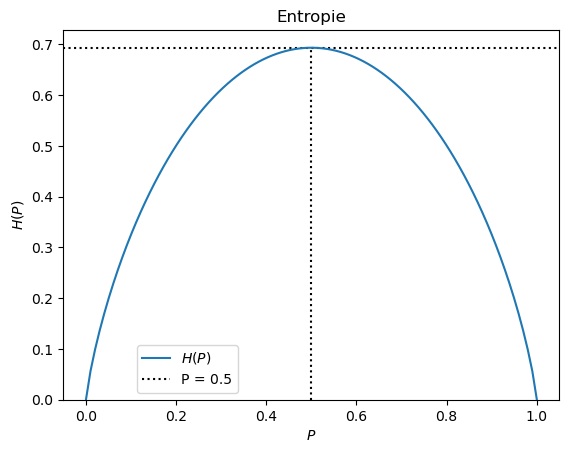
\includegraphics[width=1.0\linewidth]{Images/entropie}
				\label{fig:entropie}
			\end{figure}			
		\end{column}
		\begin{column}{0.5\textwidth}
			In the adjacent plot:
			\begin{itemize}
				\item We see that the entropy reaches a maximum value when the coin is perfectly fair: $P = 0.5$.
				\item We also see that the entropy becomes zero when the surprise is zero: $P = 0$ or $P = 1$.
			\end{itemize}
		\end{column}
	\end{columns}	
\end{frame}

\subsection[Cross-Entropy]{Cross-Entropy}

\begin{frame}{Intuition of Cross-Entropy}
	Let us perform another experiment. I have a coin, but you do not know the true probability $P(X = \text{"Tails"})$. I tell you that the probability of getting "Tails" is 0.7. I denote this probability as $Q(X = \text{"Tails"}) = 0.7$; this is the information I communicated to you:
	\pause
	\begin{itemize}
		\item I flip the coin once, and the result is "Tails".
		\item Now you know how to calculate the surprise associated with this result:
		\begin{equation*}
			I(X = \text{"Tails"}) = - \log{0.7} \approx 0.357
		\end{equation*}
	\end{itemize} 
\end{frame}

\begin{frame}{Intuition of Cross-Entropy}
	\begin{itemize}
		\item I repeat this experiment multiple times so that you can compute an expected value of the surprise.
		\pause
		\item However, there is a difference between the \textbf{true} probability of a flip resulting in "Tails" and the probability you used to compute the surprise, which corresponds to the probability I \textbf{communicated} to you.
		\pause
		\item The calculation you performed is actually:
		\begin{equation*}
			\sum_{x \in \{\text{"Tails"}, \text{"Heads"}\}} - P(X = x) \log(Q(X = x))
		\end{equation*}
		where $P$ is the true probability and $Q$ is the communicated probability.
	\end{itemize}
\end{frame}

\begin{frame}{Definition of Cross-Entropy}
	\begin{block}{Definition: Cross-Entropy}
		The cross-entropy, denoted by $H(P, Q)$, between two probability distributions $P$ and $Q$ is defined as:
		\begin{equation*}
			H(P,Q) = \mathbb{E}_{X \sim P}\left[I_Q(X)\right] = - \mathbb{E}_{X \sim P}\left[\log Q(X)\right]
		\end{equation*}
		$P$ represents the \textbf{true} probability of event $X$, and $Q$ represents an \textbf{estimated} probability distribution.
	\end{block}
\end{frame}

\begin{frame}{Cross-Entropy Calculation Example}
	In the previous example, we have:
	\begin{itemize}
		\item $P(X=\text{"Tails"}) = 0.8$
		\item $Q(X=\text{"Tails"}) = 0.7$
	\end{itemize}
	\pause
	The cross-entropy is therefore calculated as:
	\begin{equation*}
		\begin{aligned}
			H(P,Q)
			&= - \mathbb{E}_{X \sim P}\left[\log Q(X)\right] \\
			&= - \sum_{x} P(X = x) \log{Q(X = x)} \\
			&= - P(X = \text{"T"}) \log{Q(X = \text{"T"})} - P(X = \text{"H"}) \log{Q(X = \text{"H"})} \\
			&= - 0.8 \cdot \log{0.7} - (1 - 0.8) \cdot \log{(1 - 0.7)} \\
			&\approx 0.526
		\end{aligned}
	\end{equation*}
\end{frame}

\begin{frame}{Graphical Representation of Cross-Entropy}
	\begin{columns}
		\begin{column}{0.5\textwidth}
			\begin{figure}
				\centering
				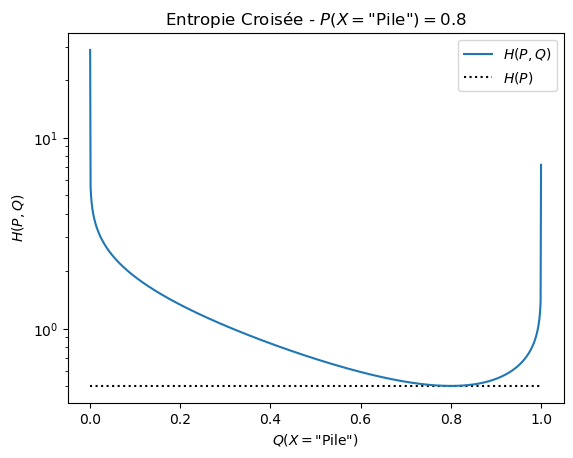
\includegraphics[width=1.0\linewidth]{Images/entropie_croisee}
				\label{fig:entropie_croisee}
			\end{figure}			
		\end{column}
		\begin{column}{0.5\textwidth}
			In the adjacent plot:
			\begin{itemize}
				\item We see that the cross-entropy reaches a minimum value when the probability $Q(X = \text{"Tails"}) = P(X = \text{"Tails"})$.
				\item This minimum value is actually the entropy: $H(P,Q) = H(P, P) = H(P)$
			\end{itemize}
		\end{column}
	\end{columns}	
\end{frame}

\begin{frame}{The Transition to Machine Learning}
	So far, we have discussed a single coin. But in a classification problem (such as predicting whether a rugby player is a forward), we do not have 1 player tested $n$ times, but rather $n$ different players.
	
	\pause
	\vspace{0.3cm}
	It is as if we had a bag containing \textbf{$n$ entirely different coins} (different sizes, weights, metals...).
	\pause
	\begin{itemize}
		\item \textbf{The features:} The physical properties of coin $i$ represent our variables $X^{(i)}$.
		\item \textbf{The prediction:} The model observes coin $i$ and predicts a probability $q^{(i)}$.
		\item \textbf{The reality:} We flip coin $i$ exactly once, and the true result is $y^{(i)} \in \{0, 1\}$.
	\end{itemize}
\end{frame}

\begin{frame}{The Surprise for a Specific Coin}
	For a given coin $i$ in our dataset, we already know the outcome (the label $y^{(i)} \in \{0, 1\}$).
	\pause
	\begin{itemize}
		\item Since the outcome is known and certain, the \textbf{empirical} probability $\hat{P}$ for this coin is exactly equal to its label $y^{(i)}$.
		\item The model, however, outputs an \textbf{estimated} probability $Q$ denoted as $q^{(i)}$.
	\end{itemize}
	\pause
	\vspace{0.3cm}
	We can therefore write the model's surprise for this coin by replacing $\hat{P}$ with $y^{(i)}$ and $Q$ with $q^{(i)}$:
	\begin{equation*}
		I_Q^{(i)} = - \left[ y^{(i)} \log(q^{(i)}) + (1 - y^{(i)}) \log(1 - q^{(i)}) \right]
	\end{equation*}
\end{frame}

\begin{frame}{The Loss Function}
	To evaluate the overall performance of our model across the entire bag of coins, we compute its \textbf{average surprise} over the $n$ coins.
	\pause
	The average cross-entropy, also called empirical cross-entropy or log-loss, is then naturally written as:
	\begin{equation*}
		H(\hat{P}, Q) 
		= - \frac{1}{n} \sum_{i=1}^n \left[ y^{(i)} \log{\left(q^{(i)}\right)} + (1 - y^{(i)}) \log{\left(1 - q^{(i)}\right)} \right]
	\end{equation*}
	\pause
	Training our logistic regression model amounts to finding the parameters that make the model \textbf{as least surprised as possible} on average when it discovers the reality of our $n$ examples!
\end{frame}

\begin{frame}{Relative Entropy}
	\begin{block}{Definition: Relative Entropy}
		Relative entropy, or the Kullback-Leibler divergence (sometimes simply abbreviated as the KL divergence), is the difference between cross-entropy and entropy:
		\begin{equation*}
			D_{\text{KL}}(P \parallel Q) = H(P,Q) - H(P)
		\end{equation*}
		Note: this difference is not symmetric:
		\begin{equation*}
			D_{\text{KL}}(P \parallel Q) \ne D_{\text{KL}}(Q \parallel P)
		\end{equation*}
	\end{block}
\end{frame}

\begin{frame}{Relative Entropy}
	\begin{itemize}
		\item \textbf{Entropy}: measures the intrinsic entropy of the individual.
		\item \textbf{Cross-entropy}: adds an additional entropy due to a poor estimation to the intrinsic entropy.
		\item \textbf{KL divergence}: measures only the additional entropy due to the poor estimation.
	\end{itemize}
	\pause
	\vspace{0.5cm}
	Even if we do not use the KL divergence explicitly by name, seeking a minimum cross-entropy (or a maximum log-likelihood) in a classification problem is actually equivalent to finding a model that makes the KL divergence as close to 0 as possible. It is therefore a fundamental concept in machine learning.
\end{frame}

\begin{frame}{Summary: Entropy, Cross-Entropy, Relative Entropy}
	\begin{itemize}
		\item \textbf{Entropy}: is the fundamental concept at the heart of decision trees.
		\item \textbf{Cross-entropy}: naturally stems from entropy when surprise is calculated using an estimated probability rather than the true probability. This allowed us to bridge the connection with the loss function of logistic regression, which will also be the loss function for neural networks in classification problems.
		\item \textbf{KL divergence}: specifically measures the entropy added because of the probability estimation. We will also use it in the neural networks course as a penalty in the loss function.
	\end{itemize}
\end{frame}